% Bibliography is maintained in references.bib.

\documentclass{thesis-library}
   
\usepackage{lipsum}
\usepackage{float}
\usepackage{url}
\renewcommand{\UrlFont}{\ttfamily\small}

% Unified screenshot command - produces identical full-width framed boxes for all figures
\newcommand{\screenshot}[1]{%
  \IfFileExists{#1}{%
    \fbox{\includegraphics[width=\dimexpr\linewidth-2\fboxsep-2\fboxrule\relax]{#1}}%
  }{%
    \fbox{\parbox[c][5cm][c]{\dimexpr\linewidth-2\fboxsep-2\fboxrule\relax}{%
      \centering\small Screenshot not available}}%
  }%
}

% Abbreviations List
\newacronym{dms}{DMS}{Donation Management System}
\newacronym{cse}{CSE}{Computer Science and Engineering}

% Variable
\newcommand{\projectTitle}{\textbf{Donation Management System}}

\begin{document}
\justifying
\newcommand{\thesisTitle}{Campus Based Donation Management System}

\newcommand{\byLabel}{\underline{Submitted By}}
\newcommand{\studentID}{Student ID: 200114}
\newcommand{\studentRegYear}{Registration Year: 2020-21}
\newcommand{\studentName}{Ramjan Ali Kha}
\newcommand{\supervisorLabel}{\underline{Supervisor}}
\newcommand{\supervisorName}{Dr. Mohammad Nowsin Amin Sheikh}
\newcommand{\supervisorDesig}{Assistant Professor}
\newcommand{\supervisorAff}{Department of Computer Science and Engineering}
\newcommand{\degreeLineALabel}{This project report was submitted in partial fulfillment of the}
\newcommand{\degreeLineBLabel}{Requirements for the BSc.Engg Degree}
\newcommand{\majorName}{In \textbf{Computer Science and Engineering.}}
\newcommand{\universityName}{Jashore University of Science and Technology}
\newcommand{\regionName}{Jashore-7408, Bangladesh}
\newcommand{\degreeyearName}{2026}
\newcommand{\degreemonthName}{April}
\newcommand{\approvalText}{This project titled \textbf{Campus Based} \textbf{Donation Management System}
submitted by \textbf{Ramjan Ali Kha} for final defence for the degree of B.Sc. in Computer Science and
Engineering on April 27, 2025.}
\newcommand{\studentSign}{\underline{Signature of the Student}}
\newcommand{\supervisorSign}{\underline{Signature of the Supervisor}}

\makecoverpage
\makeapprovalpage

\pagenumbering{roman}

\chapter*{Acknowledgments}
\addcontentsline{toc}{chapter}{Acknowledgments}
I want to thank \textbf{Almighty Allah}, the Creator and the Sustained of the word, for providing us with the opportunity, capacity, energy, spirit, and patience to finish the report.
\\
I want to express my sincere gratitude to Dr. Mohammad Nowsin Amin Sheikh, assistant professor at Jashore University of Science and Technology and my respected educator and supervisor. His unwavering advice and direction were crucial to the success of this project. In order to make this project writing as perfect as possible, he was constantly offering valuable assistance. The completion of the report would not have been possible without his extensive knowledge, insightful ideas, boundless enthusiasm, invaluable advice, assistance, and suggestions. I am honored to have had the chance to work and study under his supervision.
\\
I also want to express my gratitude to the honorable faculty of the Department of Computer Science and Engineering. I appreciate their support and helpful criticism, which enabled me to write my project report more skillfully.
\\
My friends and family have been a major source of inspiration and passion for me, and for that I am incredibly grateful. All of their love, kindness, and support have been invaluable to me during this time.
\\
I would want to thank my parents and family for their unwavering support and motivation. I am grateful for your understanding, love, support, and patience, all of which inspired me to complete my studies.

\listofabbreviations

\tableofcontents

\newpage
\listoffigures
\newpage
\listoftables
\newpage
\chapter*{List of Acronyms}
\vspace{-40pt}
\begin{table}[h]
    \renewcommand{\arraystretch}{1.6}
    \centering
    \caption{List of Acronyms.}
    \vspace{10pt}
    \begin{tabularx}{\linewidth}{|l|L|}
        \hline
        \textbf{Acronyms} & \textbf{Full Form} \\
        \hline
        DMS & Donation Management System\\
        UI & User Interface\\
        API & Application Programming Interface\\
        CRUD & Create, Read, Update, Delete\\
        JWT & JSON Web Token\\
        ORM & Object-Relational Mapping\\
        REST & Representational State Transfer\\
        HTTPS & Hypertext Transfer Protocol Secure\\
        SQL & Structured Query Language\\
        EF & Entity Framework\\
        RBAC & Role Based Access Control\\
        HTML & Hypertext Markup Language\\
        CSS & Cascading Style Sheets\\
        TypeScript & Programming Language\\
        React & JavaScript Library\\
        Redux & State Management\\
        .NET & Framework\\
        C\# & Programming Language\\
        \hline
    \end{tabularx}
\end{table}

\chapter*{Abstract}
\addcontentsline{toc}{chapter}{Abstract}
Effective philanthropic administration demands the seamless coordination of fundraising campaigns, transparent allocation of resources, rigorous volunteer management, and accountable financial stewardship. Despite this, a significant number of charitable organizations, particularly those operating within academic institutions, continue to depend on paper-based record-keeping and fragmented manual workflows. The limitations of such approaches became especially evident during participation in two campus fundraising initiatives: the 2024 Sylhet flood relief campaign and the collection drive for the medical expenses of our late sister Atika (CSE 17-18). In both cases, the reliance on manual processes introduced data inaccuracies, obscured fund utilization, and imposed unnecessary procedural overhead. These direct observations provided the central motivation for the development of the Donation Management System (DMS) presented in this report. The DMS is a consolidated web-based platform designed to unify and automate the full spectrum of donation-related operations.
\\
The system adopts a multi-tier architectural design. At the application layer, an ASP.NET Core Web API implements business logic and exposes RESTful service endpoints. The presentation layer is developed using React coupled with TypeScript, yielding a responsive and statically typed user interface. Persistent data storage is managed through Entity Framework Core atop a relational database, ensuring maintainable schema evolution as the project matures.
\\
Security considerations have been embedded across every layer of the architecture. Password credentials are protected through BCrypt hashing, cross-site request forgery is mitigated via token-based safeguards, all input is subject to server-side validation, and monetary transactions are processed exclusively through a secured payment gateway. A responsive design strategy further ensures cross-device interoperability, from desktop workstations to mobile handsets. Collectively, these measures substantially reduce manual intervention, strengthen the transparency of donation tracking, and simplify the end-to-end management of fundraising operations.
\\
The platform's feature set encompasses campaign lifecycle management, both online and physical donation processing, volunteer coordination, role-based access control, automated sentiment analysis of donor testimonials, and in-kind contribution tracking with OTP-based verification. The principal objective is to cultivate donor confidence through operational visibility and to accelerate organizational workflows through targeted automation.


\newpage
\pagenumbering{arabic}

\printchaptertitle{Introduction}
\newpage
\section{Overview}
The \textbf{Campus Based Donation Management System} constitutes a web-based software architecture conceived to digitize and systematize the administrative processes governing institutional philanthropy \cite{robinson2019digital,sander2021digital}. By unifying administrators, donors, and volunteers within a single digital ecosystem, the platform introduces role-differentiated interfaces that substantially mitigate the logistical inefficiencies characteristic of paper-dependent coordination models.

Functionally, the system addresses three principal operational domains:
\begin{itemize}
    \item \textbf{Financial Administration:} Real-time monitoring of donation transactions, secure online payment facilitation through SSLCommerz \cite{hossain2019e}, and physical donation authentication via One-Time Password (OTP) protocols to ensure verified recording of in-kind assets.
    \item \textbf{Operational Orchestration:} Structured lifecycle management of fundraising campaigns, meritocratic progression frameworks for volunteer recognition, and formalized expenditure voucher authorization chains that replace ad-hoc approval mechanisms.
    \item \textbf{Predictive Intelligence:} An integrated machine learning subsystem capable of forecasting donation volumes, detecting transactional anomalies, and estimating donor attrition probabilities. This enables proactive rather than reactive administrative decision-making.
\end{itemize}

From an architectural standpoint, the platform adheres to a contemporary three-tier design. The presentation tier employs \textbf{React with TypeScript} \cite{freeman2021react,cherny2019programming}, ensuring a responsive and type-safe user interface. Business logic resides within an \textbf{ASP.NET Core Web API} \cite{lock2021aspnet,masse2011rest}, while data persistence is maintained through \textbf{Microsoft SQL Server} accessed via Entity Framework Core \cite{lerman2020efcore,coronel2016database}. System-wide security enforcement is achieved through JSON Web Token (JWT) authentication, BCrypt cryptographic hashing, and Role-Based Access Control (RBAC) \cite{sandhu1996rbac}. Together, these components establish a resilient and extensible foundation amenable to iterative feature expansion.

\section{Background}
Charitable organizations and campus-based donation initiatives have historically operated through manual, paper-oriented systems, or at best, loosely connected digital tools, to track contributions, coordinate campaigns, and manage volunteer personnel \cite{sander2021digital,rathore2021volunteer}. While such approaches may suffice at small scales, they become increasingly untenable as operational complexity grows. The following deficiencies, identified through both literature review and practical observation, directly informed the requirements specification for the proposed DMS:

\begin{itemize}
    \item \textbf{Tracking Latency:} Substantial delays impede the real-time monitoring of donation inflows and campaign advancement. Status information often lags behind actual conditions by hours or days, hindering timely decision-making.
    \item \textbf{Data Redundancy:} Parallel entry of identical records across disconnected spreadsheets introduces systematic inconsistencies and clerical errors. Post-hoc data cleansing is both time-intensive and prone to compounding inaccuracies.
    \item \textbf{Operational Inefficiency:} Volunteer contributions remain largely unquantified in the absence of structured tracking mechanisms. No standardized method exists for recording hours worked, tasks completed, or resource utilization.
    \item \textbf{Analytical Deficiencies:} Without dedicated analytical tools, evaluating campaign performance, identifying donor behavioral trends, or detecting declining engagement becomes prohibitively difficult.
    \item \textbf{Obstacles to Communication:} Bidirectional communication channels between organizations and their donor constituencies are frequently either informal or nonexistent, resulting in inadequate feedback loops.
    \item \textbf{Lack of Transparency:} When fund utilization remains opaque to contributors, institutional trust diminishes progressively, reducing the likelihood of sustained donor participation in subsequent initiatives.
    \item \textbf{No Financial Accountability:} Audit trails are commonly incomplete or altogether absent, precluding reliable verification that disbursed funds align with stated organizational objectives.
    \item \textbf{Limited Donor Visibility:} Donors are seldom afforded access to real-time performance indicators regarding campaign trajectories or expenditure breakdowns, which measurably discourages repeat contributions.
    \item \textbf{Absence of Physical Donation Management:} In-kind contributions (such as clothing, food, and supplies) are frequently undocumented. The resulting gaps in asset records compromise institutional accountability.
    \item \textbf{Inadequate Expense Voucher Oversight:} Campaign-related expenditures are not governed by formal voucher authorization workflows, complicating the verification and validation of operational costs.
    \item \textbf{Unregulated Fund Withdrawal Processes:} The absence of structured disbursement protocols and controlled reserve fund management elevates the risk of financial misappropriation and weakens audit trail integrity.
    \item \textbf{Absence of Predictive and Analytical Capabilities:} Conventional systems are inherently reactive; they archive historical data but provide no capacity for forecasting donation trends, identifying transactional outliers, or modeling donor attrition patterns.
    \item \textbf{Lack of Volunteer Recognition and Incentivization:} Without formalized merit-based progression and achievement recognition mechanisms, volunteer motivation and longitudinal retention are adversely affected.
    \item \textbf{Insufficient Automated Notification Infrastructure:} Critical communications, including contribution confirmations, verification credentials, and status updates, are transmitted manually, if at all, leading to delayed and unreliable stakeholder engagement.
\end{itemize}

The accelerating pace of digital transformation, coupled with rising stakeholder expectations for sophisticated online interfaces, has rendered the adoption of centralized and automated management architectures a pressing institutional necessity. The proposed Donation Management System addresses these documented shortcomings by providing a comprehensive digital framework that consolidates critical operations while upholding stringent standards of data security, financial transparency, and inclusive accessibility.

\section{Motivation}
The motivation underpinning this project stems from the recurring operational inefficiencies observed across traditional philanthropic administration workflows. Charitable organizations, particularly those embedded within academic settings, encounter persistent structural challenges across several interrelated domains:
\begin{itemize}
    \item The concurrent management of heterogeneous donation channels (spanning cash, online payments, and mobile banking) without a unified system for reconciliation.
    \item The systematic tracking of volunteer engagement and the quantitative assessment of individual contributions to organizational impact.
    \item The rigorous evaluation of campaign performance, supplemented by structured mechanisms for capturing and analyzing donor sentiment.
    \item The timely dissemination of operational updates to stakeholders and beneficiaries regarding campaign progress and fund allocation.
    \item The maintenance of secure, auditable repositories for financial transaction records and sensitive donor information.
\end{itemize}

This project endeavours to construct a scalable and extensible software framework that addresses the aforementioned bottlenecks \cite{jones2023modern}, while simultaneously establishing a stable foundation for future enhancements in philanthropic management. The adoption of contemporary web technologies and adherence to established software engineering standards ensures operational reliability, robust security enforcement, and a high degree of user satisfaction \cite{wang2021enhancing}.

\section{Problem Statement}

Organizations responsible for administering philanthropic initiatives face compound operational challenges arising from their dependence on manual processes and fragmented data management architectures \cite{barnes2018rise,sander2021digital}. These challenges manifest across several critical dimensions:
\begin{itemize}
    \item \textbf{Absence of Real-Time Monitoring:} Considerable information latency prevents both donors and administrators from tracking campaign trajectories and contribution statuses with any immediacy.
    \item \textbf{Manual Collection Vulnerabilities:} Non-automated donation procurement methods, whether cash-based or through informal transfer channels, are inherently inefficient, susceptible to clerical error, and present non-trivial security exposure.
    \item \textbf{Fragmented Volunteer Coordination:} The lack of a centralized management framework hampers the assignment of tasks, the tracking of individual engagement, and the empirical measurement of volunteer impact.
    \item \textbf{Data Integrity Degradation:} Manual record-keeping practices produce systematic data inconsistencies, undermining the reliability of reports generated for institutional oversight and decision-making.
    \item \textbf{Underdeveloped Analytical Capacity:} Administrative entities lack the diagnostic tooling required to derive actionable insights from donor behavioral data, campaign performance metrics, or stakeholder testimonial sentiment.
    \item \textbf{Security and Privacy Risks:} Conventional systems that rely on unencrypted storage media expose sensitive financial records and donor profiles to significant confidentiality and integrity threats \cite{owasp2021top10,iso27001security}.
    \item \textbf{Institutional Opacity:} Prevailing frameworks seldom incorporate transparency mechanisms; empirical evidence links donor motivation to the visible verification of fund expenditure and tangible outcome reporting.
    \item \textbf{Absence of Integrated Fiscal Accounting:} Most localized systems lack bookkeeping modules capable of synchronizing donation inflows with formal financial ledger management.
\end{itemize}

The convergence of these deficiencies underscores the imperative for an automated, web-centric management architecture: one that provides a resilient, transparent, and accountable environment for the administration of philanthropic capital and mission-driven campaign operations.

\section{Questions Addressed by the Project}

The development of the proposed system is guided by the following research questions, each of which addresses an identified gap in current donation management practice:
\begin{itemize}
    \item To what extent can a unified web-based platform enhance the efficiency of donation collection, tracking, and campaign management compared to fragmented manual approaches?
    \item What measurable advantages does role-based access control confer in multi-stakeholder donation management environments?
    \item How does real-time donation tracking influence campaign transparency and, by extension, donor satisfaction and trust?
    \item In what ways does the integration of a secure online payment gateway streamline the transactional aspects of the donation process?
    \item Can sentiment analysis applied to donor testimonials yield actionable insights into campaign impact and stakeholder sentiment?
    \item Which database management and security techniques prove most effective in safeguarding sensitive donor information within this operational context?
\end{itemize}

\newpage
\section{Objectives}
Informed by the preceding research questions, the project pursues the following principal objectives:
\begin{itemize}
    \item \textbf{To develop a unified web-based platform} that consolidates donation collection, campaign management, volunteer coordination, and reporting into a single integrated system.
    \item \textbf{To implement role-based access control} with differentiated functional permissions for Administrators, Donors, Volunteers, and Campaign Creators.
    \item \textbf{To provide real-time donation and campaign tracking} that delivers transparency and immediate feedback to all stakeholders.
    \item \textbf{To integrate secure payment processing} via the SSLCommerz gateway for reliable and efficient transaction handling.
    \item \textbf{To deliver an optimal user experience} through a responsive, intuitive interface accessible across heterogeneous device classes.
    \item \textbf{To ensure data security and integrity} through robust authentication, encryption, and server-side validation mechanisms.
    \item \textbf{To incorporate sentiment analysis} on donor testimonials as a quantitative indicator of campaign effectiveness and donor satisfaction.
    \item \textbf{To furnish comprehensive reporting and analytics} capabilities that support evidence-based decision-making and organizational performance monitoring.
\end{itemize}

\newpage
\section{Organization}

This project report is structured into six chapters, each corresponding to a distinct stage of the development process. The organization is as follows:

\textbf{Chapter 1 Introduction.} Presents the project overview, contextual background, motivating factors, problem formulation, research questions, objectives, and report structure.

\textbf{Chapter 2 Background and Related Technologies.} Surveys existing donation management solutions, examines relevant technological foundations, and identifies the functional gaps that the proposed system aims to address.

\textbf{Chapter 3 Methodology.} Details the system design approach, development process, testing strategy, deployment considerations, and security implementation.

\textbf{Chapter 4 System Architecture and Design.} Describes the frontend and backend architectures, database schema, and accompanying design artifacts including ER, Use Case, Schema, and C4 diagrams.

\textbf{Chapter 5 Implementation.} Documents the system setup, technology configuration, and implementation of key functional modules, supplemented with interface screenshots.

\textbf{Chapter 6 Conclusion and Future Work.} Summarizes the project outcomes and proposes directions for future enhancement and extension.


\printchaptertitle{Background and Related Technologies}
\section{Overview}
The progressive digitization of organizational operations has had far-reaching implications for the philanthropic sector. Donation management practices have undergone a gradual but substantive transition, moving from paper-based record-keeping and manual coordination to software-driven platforms designed to centralize campaign oversight, volunteer administration, and financial tracking. This chapter undertakes a critical examination of the prevailing approaches to donation management, surveys the principal digital platforms currently available, and delineates the technological foundations upon which the proposed Donation Management System (DMS) is constructed. The analysis culminates in the identification of specific functional and architectural gaps that the DMS is designed to remediate.

\section{Conventional Donation Management Techniques}

Conventional approaches to donation administration remain predominantly dependent on manual processes: paper-based documentation, in-person collection, spreadsheet-based tracking, and informal communication channels \cite{robinson2019digital,kalinda2022university}. Though operationally familiar and initially cost-effective, these methods introduce a well-documented set of deficiencies as organizational scale increases:

\begin{itemize}
    \item \textbf{Real-Time Monitoring Gaps:} The absence of automated data capture mechanisms results in persistent latency between actual donation activity and its reflection in organizational records. Campaign progress indicators may lag by hours or days.
    \item \textbf{Data Integrity Vulnerabilities:} Manual transcription is inherently susceptible to typographical errors, receipt misplacement, and duplicated entries, each of which degrades the reliability of downstream reporting.
    \item \textbf{Volunteer Coordination Inefficiencies:} Without centralized task assignment and progress tracking tools, the allocation and supervision of volunteer personnel becomes logistically unwieldy.
    \item \textbf{Analytical Capacity Limitations:} Spreadsheet-based environments offer minimal support for pattern recognition in donor behavior or systematic evaluation of campaign effectiveness.
    \item \textbf{Security Exposure:} Unencrypted files stored on shared network drives or personal devices present tangible risks to the confidentiality and integrity of financial and personal data.
\end{itemize}

\setlength{\parindent}{0pt}

\section{Existing Digital Donation Management Solutions}

The current landscape of donation management software comprises several platform categories, each addressing different subsets of the operational requirements identified above. A critical survey of representative solutions reveals the following:

\textbf{As-Sunnah Foundation:} Operating within a faith-based humanitarian framework, this organization maintains a proprietary digital platform oriented toward the South Asian donor base. The infrastructure integrates mobile financial services (MFS), including bKash and Nagad, to facilitate expedient resource mobilization, while employing visual evidence-based transparency mechanisms to sustain donor confidence \cite{assunnah2025digital}. Despite its effectiveness within its specific operational context, the proprietary and non-extensible nature of the platform limits its applicability to other institutional settings.

\textbf{Donorbox:} A cloud-hosted fundraising platform that provides integrated payment processing, comprehensive donor profile management, and configurable donation form interfaces \cite{barnes2018rise}. The system supports real-time transaction monitoring and automated donor communication workflows. Its capabilities are well-suited to organizations whose primary collection channel is online monetary donations, though it offers limited support for in-kind contribution tracking.

\textbf{GiveWP:} Architected as a modular WordPress plugin, GiveWP facilitates extensive form customization and ensures seamless compatibility within WordPress-based content management ecosystems. Organizations operating outside the WordPress framework derive considerably less utility from this solution.

\textbf{Network for Good:} A comprehensive fundraising coordination platform encompassing donor administration, volunteer lifecycle management, and integrated analytical reporting \cite{schlegelmilch2022strategic}. While positioned as an end-to-end solution, the associated licensing costs may render it inaccessible to resource-constrained nonprofit entities.

\textbf{Blockchain-Enabled Systems:} Emerging distributed ledger technologies demonstrate the potential to establish transparent and immutable audit trails for philanthropic transactions \cite{huang2020online}. However, the majority of blockchain-based donation systems remain at experimental stages of development and have not achieved sufficient maturity for routine operational deployment.


\subsection{Critical Limitations in Existing Solutions}

A comparative analysis of the aforementioned platforms reveals several persistent shortcomings that limit their suitability for campus-based philanthropic operations:

\begin{itemize}
    \item \textbf{Institutional Customization Deficiencies:} Commercial donation platforms are predominantly designed for general nonprofit use cases and do not accommodate the specialized workflows characteristic of academic and campus environments, where students, faculty, and external donors interact through distinct operational channels.
    \item \textbf{Financial Accessibility Barriers:} Subscription-based pricing models and elevated licensing fees restrict access for student-managed organizations with constrained budgets \cite{sanchez2019framework}.
    \item \textbf{Integration Constraints:} Established platforms frequently lack interoperability pathways with existing institutional systems, including student information databases and university financial software.
    \item \textbf{Analytical Superficiality:} Few commercial solutions offer predictive analytical capabilities such as donation trend forecasting or donor attrition modeling; most are limited to retrospective reporting.
    \item \textbf{In-Kind Donation Neglect:} Physical and in-kind contributions, which are a common feature of campus-based collection drives, are inadequately supported or entirely unaddressed by prevailing platforms.
    \item \textbf{Financial Governance Gaps:} Structured expense voucher authorization workflows and controlled fund withdrawal mechanisms are largely absent from existing solutions.
\end{itemize}

\section{Role-Based Access Control in Management Systems}

Role-Based Access Control (RBAC) constitutes a foundational authorization model for multi-stakeholder digital platforms, enabling granular permission management across distinct user populations \cite{sandhu1996rbac}. Within the context of the DMS, RBAC serves several critical functions:

\begin{itemize}
    \item \textbf{Information Security Enforcement:} Access to sensitive financial records and personal data is restricted on the basis of authenticated user classification, ensuring that exposure is limited to authorized roles \cite{iso27001security}.
    \item \textbf{User Experience Optimization:} Interface customization on a per-role basis presents only contextually relevant functionality, thereby reducing cognitive load and improving task efficiency.
    \item \textbf{System Integrity Preservation:} Middleware-enforced permission checks on every incoming request prevent unauthorized data modification, including cases where requests are crafted to circumvent client-side restrictions.
    \item \textbf{Audit Trail Facilitation:} Because each action is attributed to a specific user and role, a comprehensive and traceable record of system interactions is maintained by design.
\end{itemize}

The Donation Management System implements a four-tier RBAC hierarchy comprising the following user classifications:

\begin{itemize}
    \item \textbf{System Administrators:} Granted comprehensive system access, encompassing user administration, platform configuration, financial oversight, and content moderation.
    \item \textbf{Donors:} Authorized to perform donation transactions, browse active campaigns, maintain personal profiles, submit testimonials, and retrieve receipts.
    \item \textbf{Volunteers:} Restricted to activity reporting, hour logging, individual progress tracking, and achievement visualization.
    \item \textbf{Campaign Creators:} Permitted to manage campaign lifecycles, publish progress updates, monitor fundraising trajectories, and facilitate stakeholder communication.
\end{itemize}

\section{Robust Payment Gateway Architectures}

The integration of a reliable online payment processing capability is an essential requirement for any modern philanthropic platform, necessitating robust encryption, rigorous transaction validation, and proactive fraud mitigation. SSLCommerz, a leading payment aggregator within the South Asian digital economy \cite{hossain2019e}, was selected for the DMS on the basis of its comprehensive feature set:
\begin{itemize}
    \item \textbf{Multi-Modal Payment Support:} The gateway accommodates a diverse range of payment instruments, including credit and debit cards, mobile financial services (bKash, Nagad), and internet banking, all consolidated through a unified integration interface.
    \item \textbf{Cryptographic Security Compliance:} End-to-end encryption and adherence to the Payment Card Industry Data Security Standard (PCI-DSS) ensure the confidentiality and integrity of all transaction data \cite{owasp2021top10}.
    \item \textbf{Asynchronous Transaction Verification:} Upon payment completion or failure, the gateway dispatches server-side callbacks that enable instantaneous synchronization of payment statuses without manual intervention.
    \item \textbf{Auditable Transaction Records:} Each transaction is logged at sufficient granularity to support financial reconciliation, regulatory compliance, and post-hoc audit procedures.
\end{itemize}

\section{Advanced Sentiment Analysis and Testimonial Moderation}

Sentiment analysis, a subfield of natural language processing (NLP), enables the automated extraction of evaluative indicators from unstructured textual data \cite{hutto2014vader}. Applied to donor testimonials, this capability permits organizations to derive quantitative assessments of stakeholder satisfaction and campaign impact without manual content review. Within the DMS, sentiment analysis serves the following operational functions:

\begin{itemize}
    \item \textbf{Campaign Impact Assessment:} Aggregated sentiment scores across testimonial corpora provide a quantitative measure of donor perception regarding specific campaigns and organizational initiatives.
    \item \textbf{Automated Content Moderation:} Testimonials classified with negative sentiment are automatically flagged for administrative review prior to public display, reducing moderator subjectivity and enhancing content quality assurance.
    \item \textbf{Longitudinal Satisfaction Monitoring:} Tracking sentiment distributions over time facilitates the early detection of declining donor satisfaction or emerging reputational risks.
    \item \textbf{Decision Support Integration:} Sentiment metrics, when correlated with financial and operational data, provide administrators with a more comprehensive evaluative framework for campaign strategy refinement.
\end{itemize}

The DMS enforces a mandatory administrative review gate for negatively classified testimonials before publication, thereby maintaining public-facing content integrity without imposing the overhead of exhaustive manual screening \cite{wang2021enhancing}.

\section{Modern Web Technologies}

The technological selections for the DMS were governed by considerations of framework maturity, community support breadth, and suitability for the target problem domain \cite{jones2023modern}:
\begin{itemize}
    \item \textbf{Frontend:} React with TypeScript \cite{freeman2021react,cherny2019programming,banks2017learning} provides the presentation layer, with Redux Toolkit managing centralized application state and Tailwind CSS handling responsive styling.
    \item \textbf{Backend:} ASP.NET Core Web API serves as the server-side framework, structured around RESTful service conventions with clearly separated controller and service layers.
    \item \textbf{Database:} Microsoft SQL Server provides relational data persistence, with Entity Framework Core serving as the Object-Relational Mapping (ORM) layer to abstract database operations into typed C\# code \cite{lerman2020efcore,coronel2016database}.
    \item \textbf{Authentication:} Stateless session management is implemented through JWT bearer tokens, complemented by OTP-based verification delivered via email and SMS for secondary authentication \cite{suoranta2019otp,jones2015jwt}.
    \item \textbf{Security:} Password credentials are secured via BCrypt hashing \cite{provos1999bcrypt}, form submissions incorporate CSRF token protection \cite{barth2008robust}, and all user-supplied inputs undergo server-side validation and sanitization prior to database interaction \cite{owasp2021top10}.
\end{itemize}
The selection of these technologies ensures long-term system scalability and maintainability, supported by active open-source ecosystems and well-documented upgrade pathways \cite{smith2020tech}.

\section{Advanced Features and Capabilities}

Beyond foundational donation collection and campaign management, the DMS incorporates several advanced functional modules that address persistent gaps in existing commercial platforms. These capabilities, described below, represent the principal areas of differentiation for the proposed system.

\subsection{Physical Donation Management}

The tracking and verification of in-kind and physical donations constitutes a notable omission in most conventional donation management platforms. The DMS addresses this gap through a dedicated tracking module \cite{kalinda2022university}:
\begin{itemize}
    \item \textbf{OTP-Based Donor Authentication:} Prior to the recording of any physical donation, the donor undergoes identity verification through a one-time password delivered via SMS, mitigating the risk of fraudulent or erroneous entries.
    \item \textbf{Structured Asset Documentation:} Each donated item is systematically catalogued, including descriptive metadata, estimated valuations, and temporal tracking information.
    \item \textbf{Audit Trail Maintenance:} Every physical donation event generates a verifiable record suitable for retrospective financial and compliance auditing.
    \item \textbf{Financial Ledger Integration:} In-kind contributions are synchronized with the monetary donation ledger, ensuring that aggregate campaign impact metrics remain comprehensive and accurate.
\end{itemize}

\subsection{Expense Voucher and Financial Control Systems}

Structured expenditure accounting and formalized voucher authorization workflows constitute essential financial governance mechanisms within the DMS:
\begin{itemize}
    \item \textbf{Voucher Submission and Authorization:} All campaign-related expenditures require formal documentation and hierarchical approval prior to fund disbursement, preventing unilateral spending decisions.
    \item \textbf{Attachment Management:} Supporting documentation (receipts, invoices, and procurement records) can be uploaded and associated with individual voucher entries for verification purposes.
    \item \textbf{Status Tracking:} Voucher progression through the approval workflow (submitted, under review, approved, rejected) is monitored in real time.
    \item \textbf{Automatic Ledger Synchronization:} Approved expenditures are automatically reflected in the corresponding campaign financial records.
\end{itemize}

\subsection{Withdrawal and Reserve Fund Management}

Controlled fiscal disbursement mechanisms and transparent reserve fund administration reinforce institutional financial accountability:
\begin{itemize}
    \item \textbf{Formal Withdrawal Request Workflows:} Fund disbursement follows a structured request-and-approval pipeline, ensuring that no withdrawal proceeds without administrative authorization.
    \item \textbf{Public Reserve Fund Dashboard:} A transparency-oriented dashboard displays aggregate reserve fund balances and recent transactional activity, accessible to all stakeholders.
    \item \textbf{Institutional Safeguards:} Configurable constraints and comprehensive audit trails guard against unauthorized fund depletion.
    \item \textbf{Automated Notification Infrastructure:} Relevant parties receive automated email notifications upon withdrawal approval or reserve fund status changes.
\end{itemize}

\subsection{Machine Learning Predictive Analytics}

The integration of machine learning capabilities enables evidence-based strategic planning and proactive risk identification \cite{chen2022machine,gupta2020donor}:
\begin{itemize}
    \item \textbf{Donation Demand Forecasting:} Singular Spectrum Analysis (SSA) time-series methodologies project future donation volumes across configurable temporal horizons, informing campaign resource planning \cite{hassani2007singular}.
    \item \textbf{Donor Attrition Prediction:} Binary classification algorithms identify donors exhibiting elevated disengagement risk based on recency, frequency, and monetary contribution features.
    \item \textbf{Anomaly Detection:} Statistical outlier detection methods identify transactional irregularities and atypical activity patterns within campaign donation streams \cite{ahmed2021anomaly,liu2008isolation}.
    \item \textbf{Campaign Strategy Optimization:} Insights derived from predictive models feed directly into campaign planning, enabling more informed allocation of organizational effort and resources.
\end{itemize}

\subsection{Automated Communication Infrastructure}

Timely and reliable stakeholder communication is essential for sustaining engagement and institutional credibility. The DMS automates the principal categories of outbound messaging:
\begin{itemize}
    \item \textbf{Email Notifications:} Automated dispatch of donation receipt confirmations, campaign progress updates, and administrative decision notifications.
    \item \textbf{SMS Communications:} OTP delivery for donor verification and transmission of critical system alerts through SMS channels.
    \item \textbf{Event-Driven Triggers:} The notification subsystem operates on an event-driven architecture, ensuring that communications are dispatched in temporal alignment with the triggering activities.
\end{itemize}

\printchaptertitle{Methodology}
\section{Overview}
This chapter walks through the practical steps taken to design, build, test, and secure the Donation Management System. Rather than following a rigid waterfall process, the work moved through repeated cycles by gathering requirements first then building features in small increments, testing them, and circling back to fix whatever came up. That iterative rhythm shaped most of the decisions described in the sections that follow.

\section{System Design}
At its core, the system is split into three distinct layers: a frontend client that users interact with, a backend API that handles business logic and data processing, and a relational database sitting underneath for persistent storage. Keeping these layers separate turned out to be especially useful when adding new features, since changes to one layer rarely forced changes in the others \cite{jones2023modern}.

\subsection{Key Architectural Goals}
A few non-negotiable requirements were established before any code was written:
\begin{itemize}
    \item \textbf{Modularity:} New capabilities such as a blockchain-based tracking module should plug in without disrupting what already works.
    \item \textbf{Fault Tolerance:} Payment gateways time out, databases occasionally deadlock, and the backend needed to handle both situations without crashing or leaving data in a half-updated state.
    \item \textbf{Scalability:} Campaign loads can spike dramatically during disaster relief periods. The web server and database tiers were designed so that each one could scale up independently of the other.
\end{itemize}

\subsection{Frontend Design}
We chose to build the user-facing side as a Single Page Application (SPA) using React paired with TypeScript \cite{cherny2019programming}. TypeScript catches a whole class of bugs at compile time, which saved a lot of debugging effort later on. The main design choices were:
\begin{itemize}
    \item \textbf{Responsive Layouts:} The UI relies on CSS Flexbox, Grid, and Tailwind CSS utility classes with media queries, so the same interface adjusts cleanly across phones, tablets, and desktops.
    \item \textbf{Reusable Components:} Instead of writing one-off UI code, we created shared React components for data tables, modals, and chart wrappers. This cut down on duplicated code considerably and made the interface feel more consistent.
    \item \textbf{Centralized State with Redux:} Redux Toolkit handles global state, with the store divided into feature slices like \textit{authSlice}, \textit{donorSlice}, and \textit{adminSlice} \cite{banks2017learning}. Thunk middleware manages asynchronous operations such as API calls, which keeps the components themselves simpler.
    \item \textbf{Accessibility (a11y):} WCAG guidelines were followed throughout. That meant adding ARIA attributes where needed, offering a high-contrast theme option, and making sure every interactive element is reachable through keyboard navigation alone.
\end{itemize}

Table~\ref{tab:frontend_components} gives a quick overview of how the frontend codebase is organized into layers.

\begin{table}[H]
    \centering
    \caption{Frontend Component Categorization}
    \label{tab:frontend_components}
    \vspace{10pt}
    \begin{tabularx}{\linewidth}{|P{4cm}|L|}
        \hline
        \textbf{Component Layer} & \textbf{What It Does} \\
        \hline
        Presentation Components & Stateless pieces responsible only for rendering buttons, text, cards, and similar visual elements. \\
        \hline
        Container Components & Stateful wrappers that talk to APIs, subscribe to global state, and coordinate side effects. \\
        \hline
        Routing Module & Built on React Router DOM; handles page navigation and protects routes that require authentication. \\
        \hline
        Utility Services & Shared helpers for formatting (dates, currency) and an Axios-based HTTP interceptor layer. \\
        \hline
    \end{tabularx}
\end{table}

\subsection{Backend Design}
On the server side, we went with ASP.NET Core Web API, following REST conventions for endpoint design \cite{masse2011rest}. The architecture breaks down into several clearly separated layers:
\begin{itemize}
    \item \textbf{Controllers:} These sit at the boundary of the system where they validate incoming requests, route them to the right service, and format the response. Each major feature area (authentication, campaigns, donations, payments, testimonials, volunteers, vouchers, withdrawals) has its own controller.
    \item \textbf{Services:} All the actual business logic lives here. JWT generation, payment gateway communication, email and SMS dispatch, volunteer ranking calculations, and ML predictions are all handled by dedicated service classes.
    \item \textbf{Data Transfer Objects (DTOs):} API request and response shapes are defined separately from the database entities. This keeps the API surface stable even when the underlying schema changes.
    \item \textbf{Middleware:} Cross-cutting concerns such as JWT authentication, role-based authorization, CORS policy, and serving uploaded files are configured in the ASP.NET Core middleware pipeline.
\end{itemize}

\subsection{Database Design}
Microsoft SQL Server was selected as the database engine, and Entity Framework Core serves as the ORM \cite{lerman2020efcore,coronel2016database}. Several design decisions keep the data layer reliable:
\begin{itemize}
    \item \textbf{Core Tables:} Users, Campaigns, Donations, Testimonials, VolunteerProfiles, VolunteerReports, Vouchers, ReserveFunds, and Withdrawals form the main schema.
    \item \textbf{Referential Integrity:} Foreign keys are defined explicitly, and delete behaviors (cascade, restrict, or set-null) are chosen per relationship to prevent orphaned records.
    \item \textbf{Monetary Precision:} All financial columns use \texttt{decimal(18,2)} to avoid floating-point rounding errors in accounting.
    \item \textbf{Indexed Lookups:} Frequently queried fields like user email are indexed so that lookups remain fast even as the dataset grows.
\end{itemize}

\section{Development Process}

Development was organized around Agile sprints \cite{beck2001agile,highsmith2001agile}. Each sprint lasted roughly two weeks, with a review at the end to decide what to prioritize next. This made it easy to adjust course when early testing revealed gaps in the original plan.

\subsection{Frontend Development}
Separate interfaces were built for each user role:
\begin{itemize}
    \item \textbf{Admin:} A dashboard with user management controls, analytics views, and campaign oversight tools.
    \item \textbf{Donor:} Pages for making donations, writing testimonials, and managing profile details.
    \item \textbf{Volunteer:} Screens for logging activities, tracking hours, and viewing progress within assigned campaigns.
\end{itemize}

\subsection{Backend Development}
The backend grew module by module. Here is a summary of what each module covers:
\begin{itemize}
    \item \textbf{Authentication and Authorization:} Stateless JWT-based login, email verification links, OTP-based second-factor authentication, and role-aware access control \cite{jones2015jwt}.
    \item \textbf{Donation Processing:} End-to-end donation workflows from creating the donation record through SSLCommerz payment to generating a receipt and updating campaign totals in real time.
    \item \textbf{Campaign Management:} Standard CRUD operations plus progress tracking, milestone markers, published updates, and tools for coordinating volunteers assigned to a campaign.
    \item \textbf{Physical Donation Handling:} Recording in-kind donations with item descriptions and estimated values, verifying the donor via SMS-based OTP, and syncing everything into the financial ledger.
    \item \textbf{Voucher and Expense Controls:} A voucher submission and approval pipeline, complete with document attachments and status tracking at each approval stage.
    \item \textbf{Withdrawal and Reserve Funds:} Formal withdrawal requests with admin approval, a publicly visible reserve fund dashboard, and safeguards against unauthorized fund depletion.
    \item \textbf{Sentiment Analysis:} Automated classification of testimonial text into positive, neutral, or negative categories, with mandatory admin review for anything flagged as negative.
    \item \textbf{Machine Learning:} Donation demand forecasting using Singular Spectrum Analysis, donor churn prediction, anomaly detection on donation streams, and campaign success estimation.
    \item \textbf{Analytics:} Aggregated views of donation data, campaign performance, volunteer contributions, and donor demographics with all of it exposed through dedicated API endpoints.
    \item \textbf{Notifications:} Email confirmations for donations, SMS-based OTPs, campaign update alerts, and event-triggered administrative notifications.
\end{itemize}

\section{Testing}

Both the frontend and backend were tested through a combination of automated test suites and hands-on scenario checks. The primary goal was to make sure that business logic worked correctly, API responses matched expectations, and the most important user flows did not break between releases.

\begin{table}[H]
    \centering
    \caption{Testing Matrix}
    \vspace{10pt}
    \begin{tabularx}{\linewidth}{|P{3cm}|P{3.5cm}|L|}
        \hline
        \textbf{Test Level} & \textbf{Frameworks} & \textbf{Objective} \\
        \hline
        Frontend Unit/Component & Vitest, React Testing Library & Check individual components, Redux slices, and client-side service functions in isolation. \\
        \hline
        Frontend Contract & MSW & Confirm that API wrapper functions send the right requests and handle responses correctly, using mocked endpoints. \\
        \hline
        End-to-End (E2E) & Playwright & Run through complete browser workflows like logging in, browsing campaigns, and stepping through the donation checkout. \\
        \hline
        Backend Unit/Integration & xUnit, Moq & Exercise controller and service methods under both normal and error conditions. \\
        \hline
        Security Regression & Manual API tests & Probe authorization boundaries, try malformed inputs, and verify payment callback validation. \\
        \hline
    \end{tabularx}
\end{table}

Test code lives in well-defined locations within the project:
\begin{itemize}
    \item \textbf{Frontend tests:} Found under
          \texttt{frontend/src/\allowbreak{}components/\allowbreak{}\_\_tests\_\_},
          \texttt{frontend/src/\allowbreak{}store/\allowbreak{}slices/\allowbreak{}\_\_tests\_\_},
          and \texttt{frontend/src/\allowbreak{}services/\allowbreak{}\_\_tests\_\_}.
    \item \textbf{Backend tests:} Located in
          \texttt{backend/\allowbreak{}DonationManagementSystem.\allowbreak{}Tests},
          covering both unit-level and integration-level scenarios.
    \item \textbf{Script runners:} NPM scripts group test execution into categories such as unit, contract, coverage, and E2E so they can be run selectively.
\end{itemize}

Before any release build, a lightweight PowerShell script runs backend and frontend checks locally to catch regressions early.

\section{Deployment Strategy}

Frontend and backend are packaged and deployed separately, which gives flexibility to host them on the same server or split across different environments:
\begin{itemize}
    \item \textbf{Frontend:} Vite produces an optimized static bundle that can be served by any standard web server.
    \item \textbf{Backend:} The ASP.NET Core API is published as a self-contained service; runtime settings come from \texttt{appsettings} files and environment variables.
    \item \textbf{Database:} Schema changes are handled via EF Core migrations, with automatic checks on application startup to ensure the database is up to date.
    \item \textbf{Environment Configuration:} Payment gateway credentials, JWT signing keys, and notification service settings are all injected through environment-specific configuration, keeping secrets out of source control.
\end{itemize}

\section{Security Measures}

Security was not treated as an afterthought; controls were built into every layer from the start, guided by OWASP recommendations \cite{owasp2021top10} and general information security best practices \cite{iso27001security}.

\begin{table}[H]
    \centering
    \caption{Core Security Controls}
    \vspace{10pt}
    \begin{tabularx}{\linewidth}{|P{4.5cm}|L|}
        \hline
        \textbf{Threat} & \textbf{How It Is Mitigated} \\
        \hline
        Credential compromise & Passwords are hashed with BCrypt before storage; sessions rely on short-lived JWT tokens \cite{provos1999bcrypt,jones2015jwt}. \\
        \hline
        Privilege escalation & Every protected endpoint checks the caller's role claims before executing \cite{sandhu1996rbac}. \\
        \hline
        Payment callback tampering & Callback payloads from SSLCommerz are validated server-side before any financial records are updated. \\
        \hline
    \end{tabularx}
\end{table}

A more detailed breakdown of the security layers:
\begin{itemize}
    \item \textbf{Authentication:} JWT bearer tokens with configurable issuer, audience, and expiry windows \cite{jones2015jwt}. Refresh tokens allow seamless session renewal without forcing a re-login.
    \item \textbf{Password Storage:} All passwords go through BCrypt hashing; password-reset tokens are verified against stored hashes as well \cite{provos1999bcrypt}.
    \item \textbf{Authorization:} RBAC policies restrict what each role can access so admin-only endpoints are unreachable for donor or volunteer accounts \cite{sandhu1996rbac}.
    \item \textbf{Input Validation:} Incoming data is validated server-side through DTO model annotations and controlled update flows, preventing injection and malformed-data attacks.
    \item \textbf{Network and Asset Security:} CORS is configured to accept requests only from known origins, and uploaded files are served from controlled static-file paths rather than arbitrary locations.
\end{itemize}

\printchaptertitle{System Architecture and Design}
\section{Overview}
This chapter lays out how the system is structured from the frontend and backend layers down to the database tables and includes the diagrams used to document the design. Rather than repeating the methodology details from the previous chapter, the focus here is on the concrete architectural decisions and the resulting data model.

\section{Frontend Architecture}
The client side is built around React's component model, with a few key technologies holding it together:
\begin{itemize}
    \item React components handle all UI rendering and user interaction.
    \item A Redux store provides one centralized place for application-wide state.
    \item Tailwind CSS takes care of styling and responsive behavior.
    \item TypeScript adds static type checking, which helps catch mistakes before they reach the browser.
\end{itemize}

\section{Backend Architecture}
The server-side API is written in .NET Core and sticks to RESTful design principles \cite{masse2011rest}. Its internal structure keeps different responsibilities cleanly separated:
\begin{itemize}
    \item \textbf{Controllers:} Accept HTTP requests, validate inputs, and return properly formatted responses. Each feature module has a dedicated controller.
    \item \textbf{Services:} Where the business rules actually live. Domain operations, cross-module coordination, and anything requiring non-trivial logic are handled at this layer.
    \item \textbf{Data Access:} Entity Framework Core, via the \texttt{AppDbContext} class, manages database queries and persistence.
    \item \textbf{Middleware:} Handles concerns that cut across the whole application: authentication checks, authorization enforcement, CORS policies, and serving uploaded files.
    \item \textbf{DTOs:} Request and response shapes are defined as separate data contracts, so internal schema changes do not automatically break the external API surface.
\end{itemize}

\section{Database Schema and Data Dictionary}
All persistent data lives in a SQL Server database, with Entity Framework Core managing the schema through code-first migrations \cite{coronel2016database}. The tables below are representative of the core data model.

\subsection{Table Campaigns}
{\RaggedRight
This table drives the entire fundraising lifecycle covering creation, progress tracking, and eventual completion or cancellation.\par}
\begin{table}[H]
    \centering
    \caption{Data Dictionary - Campaigns Entity}
    \vspace{10pt}
    \begin{tabularx}{\linewidth}{|l|l|l|L|}
        \hline
        \textbf{Column Name} & \textbf{Data Type} & \textbf{Constraint} & \textbf{Description} \\
        \hline
        Id & INT & PRIMARY KEY & Auto-increment campaign identifier. \\
        \hline
        Title & NVARCHAR(200) & NOT NULL & Campaign title displayed to donors. \\
        \hline
        TargetAmount & DECIMAL(18,2) & NOT NULL & Goal numerical value. \\
        \hline
        AmountRaised & DECIMAL(18,2) & DEFAULT(0.0) & Cumulatively dynamically updated value. \\
        \hline
        Status & NVARCHAR(50) & NOT NULL & State such as pending, active, completed, cancelled. \\
        \hline
        CreatedBy & INT & FOREIGN KEY & User who created the campaign. \\
        \hline
        CreatedAt & DATETIME2 & DEFAULT(GETDATE()) & Record creation timestamp. \\
        \hline
    \end{tabularx}
\end{table}

\subsection{Table Donations}
{\RaggedRight
Each row here records a single donation transaction, linking a donor to a specific campaign.\par}
\begin{table}[H]
    \centering
    \caption{Data Dictionary - Donations Entity}
    \vspace{10pt}
    \begin{tabularx}{\linewidth}{|l|l|l|L|}
        \hline
        \textbf{Column Name} & \textbf{Data Type} & \textbf{Constraint} & \textbf{Description} \\
        \hline
        Id & INT & PRIMARY KEY & Donation record identifier. \\
        \hline
        CampaignId & INT & FOREIGN KEY & Parent campaign reference. \\
        \hline
        UserId & INT (nullable) & FOREIGN KEY & Registered donor reference (nullable for guest donations). \\
        \hline
        Amount & DECIMAL(18,2) & NOT NULL & Donation amount. \\
        \hline
        PaymentReference & NVARCHAR(MAX) & NULLABLE & Gateway transaction reference value. \\
        \hline
        Status & NVARCHAR(50) & NOT NULL & pending, completed, failed, or refunded. \\
        \hline
    \end{tabularx}
\end{table}

\subsection{Table Volunteer Reports}
{\RaggedRight
Volunteers can file reports about misconduct, no-shows, or other issues against fellow volunteers. This table stores those reports along with their review status.\par}
\begin{table}[H]
    \centering
    \caption{Data Dictionary - Volunteer Reports}
    \vspace{10pt}
    \begin{tabularx}{\linewidth}{|l|l|l|L|}
        \hline
        \textbf{Column Name} & \textbf{Data Type} & \textbf{Constraint} & \textbf{Description} \\
        \hline
        Id & INT & PRIMARY KEY & Report identifier. \\
        \hline
        ReportedByVolunteerId & INT & FOREIGN KEY & Volunteer profile that submitted the report. \\
        \hline
        ReportedVolunteerId & INT & FOREIGN KEY & Volunteer profile being reported. \\
        \hline
        ReportType & NVARCHAR(MAX) & NOT NULL & Type such as misconduct, no-show, or other. \\
        \hline
        Description & NVARCHAR(MAX) & NOT NULL & Detailed narrative of the incident. \\
        \hline
        Status & NVARCHAR(MAX) & NOT NULL & pending, under\_review, resolved, or rejected. \\
        \hline
    \end{tabularx}
\end{table}

Beyond these three core tables, the database includes several other entities that round out the platform:
\begin{itemize}
    \item \textbf{Users:} Stores identity data, assigned roles, and profile information.
    \item \textbf{Testimonials:} Holds donor feedback along with computed sentiment scores and moderation flags.
    \item \textbf{CampaignUpdates:} Contains progress posts and milestone announcements published by campaign creators.
    \item \textbf{PhysicalDonations:} Tracks in-kind contributions collected by volunteers, with OTP verification records.
    \item \textbf{Vouchers, ReserveFunds, Withdrawals:} Together, these tables manage expense approval workflows, reserve fund balances, and controlled disbursements.
\end{itemize}

\section{ER Diagram}
The ER diagram below maps out the relationships between entities with one-to-many links between Users and Donations, Campaigns and Donations, and so forth.

\begin{figure}[H]
    \centering
    \screenshot{images/er_diagram.png}
    \caption{Entity-Relationship Diagram.}
\end{figure}

\section{Use Case Diagram}
The use case diagram below shows which actions are available to each role. Admins have the broadest access, while Donors, Volunteers, and Campaign Creators each see a focused subset of the system:

\begin{figure}[H]
    \centering
    \screenshot{images/use_case_diagram.png}
    \caption{Use Case Diagram.}
\end{figure}

\section{Schema Diagram}
This diagram provides a closer look at every table in the database, including column names, data types, and the foreign key connections between them:

\begin{figure}[H]
    \centering
    \screenshot{images/schema_diagram.png}
    \caption{Database Schema Diagram.}
\end{figure}

\section{System Context Diagram}
At the highest level of the C4 model (Level 1), we can see the DMS interacting with external actors and external systems like SSLCommerz and email/SMS providers.

\begin{figure}[H]
    \centering
    \screenshot{images/system_context_diagram.png}
    \caption{System Context Diagram.}
\end{figure}

\section{Container Diagram}
Going one level deeper (C4 Level 2), the container diagram breaks the system into its major runtime pieces: the React SPA, the .NET API, the SQL Server database, and the third-party services it depends on.

\begin{figure}[H]
    \centering
    \screenshot{images/container_diagram.png}
    \caption{Container Diagram.}
\end{figure}

\section{Component Diagram}
Inside the backend container, the component diagram shows how controllers, services, and data-access classes connect to one another.

\begin{figure}[H]
    \centering
    \screenshot{images/component_diagram.png}
    \caption{Component Diagram.}
\end{figure}

\section{Class Diagram}
A simplified class diagram captures the main domain objects such as Users, Campaigns, and Donations and the relationships between them.

\begin{figure}[H]
    \centering
    \screenshot{images/class_diagram.png}
    \caption{Class Diagram.}
\end{figure}

\section{Data Flow Diagram (Level 0)}
The Level~0 DFD draws a boundary around the entire system, showing external entities (donors, admins, payment gateway) and the high-level data stores they interact with.

\begin{figure}[H]
    \centering
    \screenshot{images/dfd_level0_diagram.png}
    \caption{Data Flow Diagram (Level 0).}
\end{figure}

\section{Data Flow Diagram (Level 1)}
Drilling into Level~1, the major process is split into module-level groups like authentication, donations, campaigns, and analytics while the data movements between them become visible.

\begin{figure}[H]
    \centering
    \screenshot{images/dfd_level1_diagram.png}
    \caption{Data Flow Diagram (Level 1).}
\end{figure}

\section{Deployment Diagram}
The deployment diagram maps each software container to the infrastructure node that hosts it, along with connections to external integrations.

\begin{figure}[H]
    \centering
    \screenshot{images/deployment_diagram.png}
    \caption{Deployment Diagram.}
\end{figure}

\section{Activity Diagram: Donation Workflow}
This activity diagram traces what happens from the moment a donor clicks ``Donate'' to the final status update covering payment initiation, gateway redirect, callback processing, and record finalization.

\begin{figure}[H]
    \centering
    \IfFileExists{images/donation_activity_diagram.png}{%
        \fbox{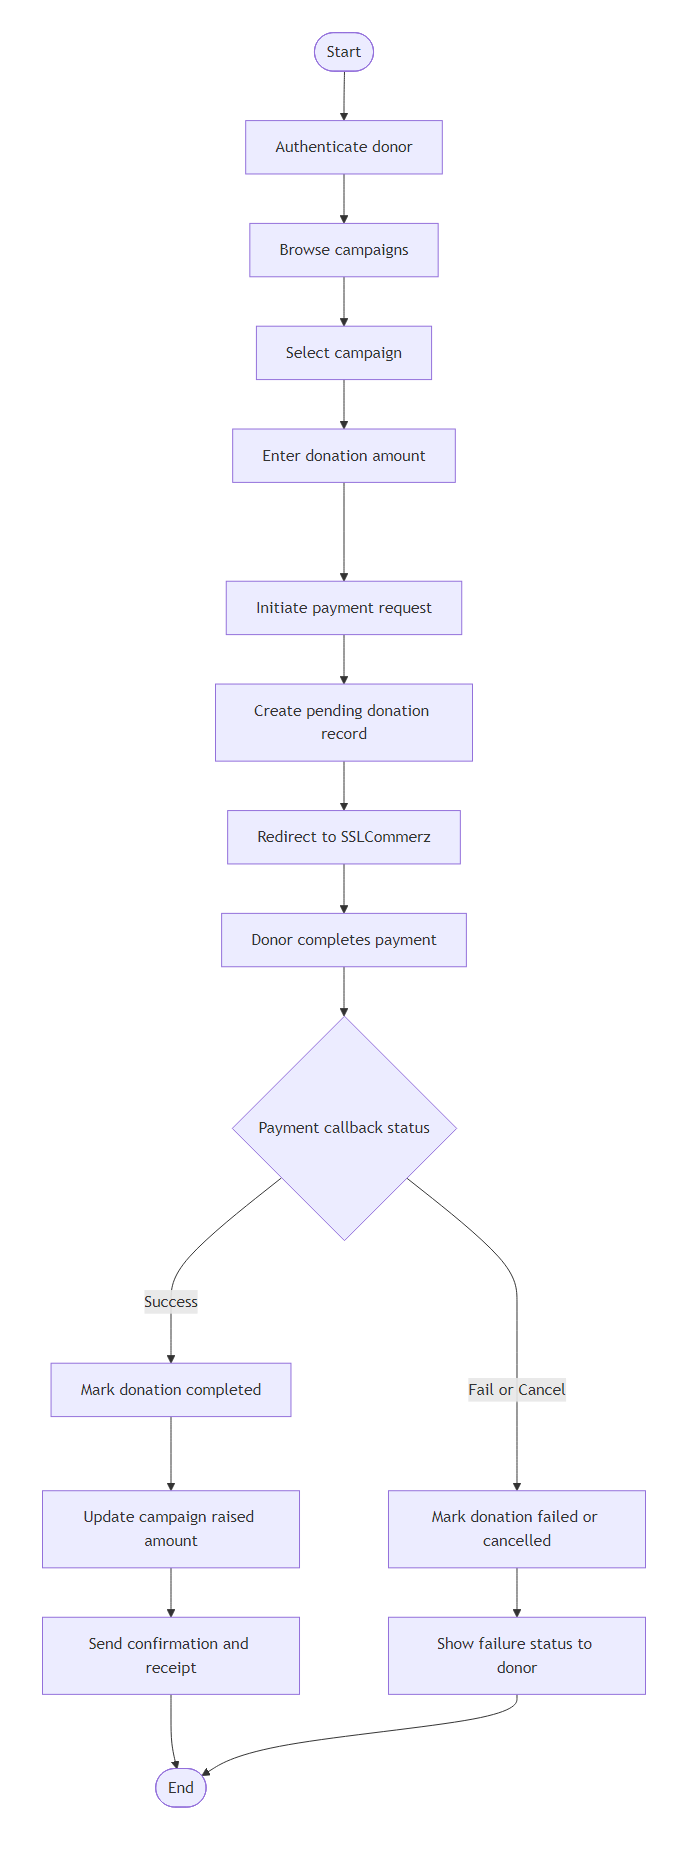
\includegraphics[%
            width=\dimexpr\linewidth-2\fboxsep-2\fboxrule\relax,%
            height=0.88\textheight,%
            keepaspectratio%
        ]{images/donation_activity_diagram.png}}%
    }{%
        \fbox{\parbox[c][5cm][c]{\dimexpr\linewidth-2\fboxsep-2\fboxrule\relax}{%
            \centering\small Donation activity diagram image not available}}%
    }
    \caption{Activity Diagram for Donation Workflow.}
\end{figure}

\section{Campaign Lifecycle State Diagram}
Campaigns move through a defined set of states such as pending approval, active, completed, and cancelled with only certain transitions allowed. The diagram below formalizes those rules.

\begin{figure}[H]
    \centering
    \screenshot{images/campaign_state_diagram.png}
    \caption{Campaign Lifecycle State Diagram.}
\end{figure}

\section{Authentication Flow}
Authentication relies on JWTs with role-aware authorization \cite{jones2015jwt}. Here is how the process works in practice.

\subsection{Registration, Login, and Token Issuance}
\begin{enumerate}
    \item When a new user registers, their password is hashed with BCrypt and stored never in plain text \cite{provos1999bcrypt}.
    \item An email verification token is generated and sent to the user's inbox.
    \item At login, the server verifies credentials and returns both a JWT access token and a refresh token.
    \item When the access token expires, the refresh endpoint checks the refresh token's validity and issues a fresh access token without requiring the user to log in again.
\end{enumerate}

\subsection{Authorization and Access Control}
Once a user is authenticated, every request to a protected endpoint goes through additional checks:
\begin{itemize}
    \item ASP.NET Core's JWT bearer middleware validates the token's signature, issuer, audience, and expiry.
    \item Claims embedded in the token are inspected to enforce role boundaries so only admin-role tokens can reach user-management endpoints \cite{sandhu1996rbac}.
    \item Profile updates and other user-specific actions require that the token's identity claim matches the target user.
\end{itemize}

\section{Payment Processing and Ledger Integration}
All monetary transactions flow through the SSLCommerz gateway, with the backend handling post-payment synchronization via callbacks \cite{hossain2019e}.

\subsection{Sequence Diagram: Payment Callback Flow}
\begin{figure}[H]
    \centering
    \screenshot{images/payment_sequence_diagram.png}
    \caption{Sequence Diagram for Donation Payment Flow.}
\end{figure}

\subsection{How a Transaction Starts}
\begin{enumerate}
    \item The donor clicks the payment button on the frontend, sending a request to the backend.
    \item \texttt{PaymentController} creates a donation record in ``pending'' status and generates a unique transaction reference.
    \item Payment metadata including amount, donor details, and callback URLs is sent to the SSLCommerz API.
    \item The user's browser is redirected to the gateway page returned by SSLCommerz.
\end{enumerate}

\subsection{Callback Handling and Idempotency}
After the donor completes (or abandons) payment, SSLCommerz sends callbacks back to the server:
\begin{itemize}
    \item The callback payload is matched to the corresponding donation via the donation ID or transaction reference.
    \item If payment succeeded, the donation's status moves from ``pending'' to ``completed.''
    \item The campaign's raised amount is incremented accordingly; any overflow beyond the target can be redirected into a reserve fund entry.
    \item Idempotency checks ensure that processing the same callback twice does not result in duplicate balance updates.
\end{itemize}

\printchaptertitle{System Implementation}

\section{System Setup}
Getting the DMS running involves two main pieces: a React-based frontend served as static files, and an ASP.NET Core backend that exposes the API and connects to the database. This section covers the technology choices and then walks through the implemented features with screenshots.

\subsection{Technologies Used}

\begin{itemize}
    \item \textbf{Frontend Technologies:}
\end{itemize}
\vspace{5pt}
\begin{table}[H]
    \centering
    \caption{Frontend Technologies.}
    \vspace{10pt}
    \begin{tabular}{|c|c|}
        \hline
        \textbf{SN} & \textbf{Technology} \\
        \hline
        1  & React \\
        2  & TypeScript \\
        3  & Redux Toolkit \\
        4  & Tailwind CSS \\
        5  & Axios (HTTP Client) \\
        6  & Vite (Build Tool) \\
        \hline
    \end{tabular}
\end{table}
\vspace{10pt}

\begin{itemize}
    \item \textbf{Backend Technologies:}
\end{itemize}
\vspace{5pt}
\begin{table}[H]
    \centering
    \caption{Backend Technologies.}
    \vspace{10pt}
    \begin{tabular}{|c|c|}
        \hline
        \textbf{SN} & \textbf{Technology} \\
        \hline
        1  & .NET Core 7/8 \\
        2  & C\# \\
        3  & Entity Framework Core \\
        4  & SQL Server \\
        5  & ASP.NET Core Identity \\
        6  & JWT Authentication \\
        \hline
    \end{tabular}
\end{table}
\vspace{10pt}

\section{System Implementation}

The screenshots below follow the same sequence a real user would encounter: logging in, navigating the admin dashboard, managing campaigns, making a donation, and so on. This ordering makes it easier to see how different parts of the system connect during actual use.

\subsection{User Authentication}
The login screen is the entry point. Behind it, JWT-based sessions handle identity, email verification ensures genuine accounts, and refresh tokens keep users logged in without repeated password prompts.

\begin{figure}[H]
    \centering
    \screenshot{images/login.png}
    \caption{Login and Authentication Interface.}
\end{figure}

\subsection{Dashboard Overview}
Once an admin logs in, the dashboard gives an at-a-glance summary: total donations collected, how many campaigns are active, items waiting for review, and recent volunteer activity.

\begin{figure}[H]
    \centering
    \screenshot{images/admin_dashboard.png}
    \caption{Admin Dashboard Overview.}
\end{figure}

\subsection{User and Role Management}
Admins can assign roles, enable or disable accounts, and manage user profiles from a dedicated panel.

\begin{figure}[H]
    \centering
    \screenshot{images/user_role.png}
    \caption{User and Role Management Panel.}
\end{figure}

\subsection{Campaign Management}
Campaign creators use this interface to set up new campaigns, define fundraising targets, upload images, post progress updates, and track how close they are to their goal.

\begin{figure}[H]
    \centering
    \screenshot{images/campaign_management.png}
    \caption{Campaign Creation and Management Interface.}
\end{figure}

\subsection{Donation Processing}
Donors go through a checkout flow that connects to SSLCommerz for payment. Once the transaction is confirmed, the system updates the donation status and campaign totals automatically.

\begin{figure}[H]
    \centering
    \screenshot{images/payment.png}
    \caption{Donation Checkout and Payment Initiation.}
\end{figure}

\subsection{Volunteer Management}
Volunteers have their own panel where they can submit activity reports, log hours, see their overall progress, and check how their contributions stack up.

\begin{figure}[H]
    \centering
    \screenshot{images/volunteer_panel.png}
    \caption{Volunteer Activity and Reporting Interface.}
\end{figure}

\subsection{Testimonial and Sentiment Analysis}
When donors leave testimonials, the system scores each one for sentiment. Negative-scoring entries are held for admin review before appearing publicly.

\begin{figure}[H]
    \centering
    \screenshot{images/testimonials.png}
    \caption{Testimonial Moderation and Sentiment Review.}
\end{figure}

\subsection{Analytics and Reporting}
The analytics dashboard pulls together donation trends, campaign performance, volunteer output, and donor activity into interactive charts and summary cards.

\begin{figure}[H]
    \centering
    \screenshot{images/analytics_dashboard.png}
    \caption{Analytics and Reporting Dashboard.}
\end{figure}

\subsection{Additional Feature Screenshots}
The remaining screenshots cover the other major modules built into the platform:

\begin{figure}[H]
    \centering
    \screenshot{images/campaign_updates.png}
    \caption{Campaign Updates and Announcement Interface.}
\end{figure}

\begin{figure}[H]
    \centering
    \screenshot{images/physical_donation.png}
    \caption{Physical Donation Verification and Tracking.}
\end{figure}

\begin{figure}[H]
    \centering
    \screenshot{images/expense_voucher.png}
    \caption{Expense Voucher Management and Approval Workflow.}
\end{figure}

\begin{figure}[H]
    \centering
    \screenshot{images/withdraw.png}
    \caption{Withdrawal Request and Approval Interface.}
\end{figure}

\begin{figure}[H]
    \centering
    \screenshot{images/reserve_fund.png}
    \caption{Reserve Fund Transparency.}
\end{figure}

\begin{figure}[H]
    \centering
    \screenshot{images/transaction_history.png}
    \caption{Payment Transaction History and Status Tracking.}
\end{figure}

\begin{figure}[H]
    \centering
    \screenshot{images/ML_insight.png}
    \caption{Machine Learning Insights and Prediction Outputs.}
\end{figure}

% \begin{figure}[H]
%     \centering
%     \screenshot{images/notification_center.png}
%     \caption{Notification and Communication Activity Interface.}
% \end{figure}

\subsection{Screenshot File Arrangement}
For consistency and maintainability, implementation screenshots should be stored under \texttt{Report/\allowbreak{}images} using the following filenames:

\begin{table}[H]
    \centering
    \caption{Implementation Screenshot Naming Scheme}
    \vspace{10pt}
    \begin{tabularx}{\linewidth}{|P{6.5cm}|L|}
        \hline
        \textbf{Filename} & \textbf{Purpose} \\
        \hline
        login\_page.png & Authentication/login screen. \\
        \hline
        admin\_dashboard.png & Main administrative overview and metrics. \\
        \hline
        user\_management.png & User, role, and access control management. \\
        \hline
        campaign\_management.png & Campaign create/update and progress monitoring. \\
        \hline
        donation\_checkout.png & Donation amount entry and payment initiation flow. \\
        \hline
        volunteer\_panel.png & Volunteer reporting and activity tracking. \\
        \hline
        testimonial\_moderation.png & Sentiment-based moderation and feedback review. \\
        \hline
        analytics\_dashboard.png & Reports and analytical visualizations. \\
        \hline
        campaign\_updates.png & Campaign announcement and progress update page. \\
        \hline
        physical\_donation.png & Physical donation collection and OTP verification workflow. \\
        \hline
        voucher\_management.png & Expense voucher submission and approval panels. \\
        \hline
        withdrawal\_management.png & Withdrawal request queue and administrative decisions. \\
        \hline
        reserve\_fund\_dashboard.png & Public reserve fund summary and transaction visibility. \\
        \hline
        payment\_transactions.png & Payment status log, callback result, and transaction history. \\
        \hline
        ml\_predictions.png & Forecasting, anomaly, and churn prediction outputs. \\
        \hline
        % \hline
        % notification\_center.png & Email/SMS/alert history and delivery status view. \\
        % \hline
    \end{tabularx}
\end{table}

\section{Key Features Implementation}

\subsection{Donation Tracking and Processing}
Donors and campaign creators can both see, in real time, how much has been raised against the target. Each individual donation is recorded with a timestamp, amount, and payment status. The processing module hooks into SSLCommerz so that payments are confirmed and receipts generated without manual intervention.

\subsection{Campaign Updates and Communications}
Campaign creators post progress updates including stories about how the funds are being used, milestone announcements, or thank-you notes. These updates keep donors informed and engaged even after they have contributed.

\subsection{Volunteer Reporting and Recognition}
Volunteers log their activities by submitting reports that include hours worked, a description of what they did, which campaign they were supporting, and any particular achievements. The system uses this data for merit-based ranking and public recognition.

\subsection{Physical Donation Management}
In-kind donations including clothes, food, and supplies are handled through a dedicated tracking module:
\begin{itemize}
    \item OTP-based donor verification via SMS.
    \item Structured item documentation and valuation.
    \item Integration with donation ledger systems.
    \item Audit trail generation for institutional accountability.
\end{itemize}

\subsection{Expense Voucher Management}
Campaign-related expenses go through a structured voucher process:
\begin{itemize}
    \item Structured voucher creation with detailed expense documentation.
    \item Hierarchical approval workflows.
    \item Supporting document attachment and verification.
    \item Real-time status monitoring and notifications.
\end{itemize}

\subsection{Financial Controls and Withdrawal Management}
Money does not leave the system without oversight:
\begin{itemize}
    \item Formal withdrawal request workflows.
    \item Administrative approval requirements.
    \item Public reserve fund transparency dashboard.
    \item Automated notification infrastructure.
\end{itemize}

\subsection{Payment Integration}
The SSLCommerz integration supports credit cards, mobile banking (bKash, Nagad), and digital wallets. Transaction confirmations are handled automatically through server-side callbacks, so neither the donor nor the admin needs to do anything manually after payment.

\subsection{Machine Learning Features}
All ML capabilities run inside the backend as an in-process \texttt{MLPredictionService} built on ML.NET. The service is registered as a singleton, which means trained models stay in memory and get reused across requests rather than being retrained every time.

\subsubsection{1. Donation Demand Forecasting (SSA)}
Weekly donation totals are fed into ML.NET's Singular Spectrum Analysis pipeline to produce forecasts with confidence bounds \cite{chen2022machine,hassani2007singular}. This gives campaign managers a rough idea of expected income over the coming weeks.

\subsubsection{2. Donor Attrition Prediction}
To identify donors who might stop contributing, the system builds a binary classification model using features like recency of last donation, total number of donations, average and total amounts, and donation frequency \cite{gupta2020donor}. The output is a probability score plus a human-readable risk label (low, medium, high) to guide re-engagement efforts.

The probability estimate is interpreted as:
\begin{equation}
    P(Attrition) = \sigma\!\left(\sum_{i=1}^{n} w_i f_i\right)
\end{equation}
where $\sigma$ denotes the sigmoid mapping to a value in $[0,1]$.

\subsubsection{3. Donation Anomaly Detection}
ML.NET's IID spike detection algorithm scans completed donation streams for outliers \cite{ahmed2021anomaly}. The kinds of things it catches include:
\begin{itemize}
    \item Single donations that are unusually large (or small) compared to the campaign's history.
    \item Sudden bursts of activity that do not match the campaign's normal pattern.
\end{itemize}
Any flagged transactions show up in the admin panel for manual review.

\subsubsection{4. Sentiment Analysis}
Testimonial text is featurized and classified using SDCA logistic regression. The model assigns each testimonial a sentiment band of positive, neutral, or negative based on confidence thresholds. Negative-scoring entries automatically enter the moderation queue \cite{hutto2014vader}.

\subsubsection{5. Campaign and Volunteer Intelligence}
The service can also estimate a campaign's probability of reaching its goal, and it recommends suitable volunteers for assignment. Volunteer recommendations are scored by combining campaign attributes (category, urgency, remaining duration) with each volunteer's profile and past activity.

\subsection{Email and SMS Notifications}
The notification system handles several types of messages:
\begin{itemize}
    \item Email-based donation receipt confirmations.
    \item Campaign update notifications.
    \item Administrative approval/rejection communications.
    \item SMS-based OTP delivery for donor verification.
    \item Real-time event-driven notifications.
\end{itemize}

\subsection{Testimonial Moderation}
As mentioned in the ML section, testimonials with negative sentiment are flagged automatically. Admins can approve, edit, or reject them before they appear on the public-facing campaign pages.

\printchaptertitle{System Evaluation and Results}

\section{System Evaluation Overview}
To check whether the system actually works as intended, we ran a combination of automated tests and manual scenario walkthroughs. The evaluation covered the main functional areas: authentication, donation workflows, volunteer features, testimonial moderation, and the analytics endpoints.

\section{Automated Test Coverage}
Both frontend and backend parts of the application have executable test suites. The table below summarizes what each layer validates.

\begin{table}[H]
    \centering
    \caption{Implemented Evaluation Layers}
    \vspace{10pt}
    \begin{tabularx}{\linewidth}{|P{4cm}|P{3.5cm}|L|}
        \hline
        \textbf{Evaluation Layer} & \textbf{Primary Tools} & \textbf{Validation Scope} \\
        \hline
        Frontend Unit/Component & Vitest, React Testing Library & UI behavior, reducers, and client service logic. \\
        \hline
        Frontend Contract & MSW & Contract-level checks for API wrapper behavior and payload handling. \\
        \hline
        Backend Unit/Integration & xUnit, Moq & Controller and service behavior under success and error conditions. \\
        \hline
        End-to-End & Playwright & End-user flows from login through dashboard and donation paths. \\
        \hline
    \end{tabularx}
\end{table}

\section{Functional Validation Scenarios}
The most critical business workflows were tested through a mix of API-level checks and manual end-to-end runs:

\begin{table}[H]
    \centering
    \caption{Critical Workflow Validation}
    \vspace{10pt}
    \begin{tabularx}{\linewidth}{|P{6.5cm}|l|L|}
        \hline
        \textbf{Workflow} & \textbf{Validation Type} & \textbf{Expected Outcome} \\
        \hline
        Registration and login & Automated + manual & Valid account creation, token issuance, and protected-route access. \\
        \hline
        Donation and payment callback & Manual integration & Pending donation updates to completed on successful callback. \\
        \hline
        Volunteer and reporting modules & API + UI checks & Report submission and status transitions operate correctly. \\
        \hline
        Testimonial moderation and analytics & API tests & Sentiment analysis and moderation states are persisted and retrievable. \\
        \hline
    \end{tabularx}
\end{table}

\section{ML Endpoint Validation}
Each ML capability is exposed through a dedicated API endpoint in \texttt{MLController}. During evaluation, we hit each endpoint with representative data and verified the outputs:
\begin{itemize}
    \item \textbf{Forecasting:} Weekly donation forecasts with confidence intervals.
    \item \textbf{Sentiment:} Text scoring and class mapping (positive/neutral/negative).
    \item \textbf{Donor Churn:} Risk scoring based on donor activity history.
    \item \textbf{Campaign Success:} Probability estimate for campaign goal completion.
    \item \textbf{Anomaly Detection:} Outlier reporting for campaign donation streams.
\end{itemize}

\section{Limitations and What Comes Next}
This round of evaluation focused mainly on whether things work correctly and whether regressions are caught. What it does not yet cover is performance under load because we have not run formal benchmarks in a production-like environment. The ML models would also benefit from validation against larger historical datasets, which were not available during the project timeline.

\printchaptertitle{Conclusion and Future Work}

\section{Conclusion}

Looking back at what we set out to build, the Donation Management System has turned into a fairly full-featured platform. It covers the core operations that any campus-based charity effort would need including collecting donations, running campaigns, coordinating volunteers, and keeping financial records transparent while also adding some capabilities that existing solutions tend to miss, like in-kind donation tracking with OTP verification and ML-based analytics.

A quick summary of what the system delivers:
\begin{itemize}
    \item \textbf{Donation Processing:} Secure, real-time payments through SSLCommerz with automatic receipt generation and campaign total updates.
    \item \textbf{Campaign Visibility:} Live progress tracking, published updates, and a public reserve fund view so that donors can see exactly where money goes.
    \item \textbf{Volunteer Support:} Activity logging, hour tracking, and a ranking system that rewards consistent contributors.
    \item \textbf{ML-Driven Insights:} Donation forecasting, anomaly detection, donor churn scoring, and sentiment analysis all running inside the backend without external dependencies.
    \item \textbf{Financial Controls:} Expense vouchers require approval before funds are released, withdrawals go through a formal request pipeline, and everything leaves an audit trail.
    \item \textbf{Physical Donation Tracking:} In-kind contributions are documented, valued, and linked to the ledger.
    \item \textbf{Testimonial Moderation:} Automated sentiment scoring flags risky content for admin review before publication.
    \item \textbf{Access Control:} RBAC makes sure each user type (admin, donor, volunteer, campaign creator) sees only what they should.
    \item \textbf{Cross-Device Access:} The UI works on phones, tablets, and desktops, following accessibility guidelines throughout.
\end{itemize}

The technology stack of ASP.NET Core, React with TypeScript, SQL Server, and Redux Toolkit has held up well. It is mature enough for a production deployment and flexible enough to grow.  Security was baked in early: JWT authentication, BCrypt password hashing, server-side input validation, and CORS restrictions are all in place. None of this is exotic, but it covers the OWASP essentials and goes a long way toward earning donor trust.

If nothing else, this project has shown that the manual, spreadsheet-driven approach to campus fundraising can realistically be replaced with software. The result is more transparent, less error-prone, and honestly just easier for everyone involved.

\section{Future Work}

The current system is functional, but there is plenty of room to grow. Some directions worth pursuing:

\begin{itemize}
    \item \textbf{Multilingual Support:} Translating the interface and notification messages into Bangla and other languages would make the platform more accessible. Sentiment analysis would also need to work across languages.
    \item \textbf{Better ML Models:} The current models are a solid starting point, but training on larger, real-world datasets and experimenting with deeper architectures (neural networks, for example) could improve forecast accuracy and churn prediction.
    \item \textbf{Blockchain Transparency:} A distributed ledger layer could provide tamper-proof donation records, which is increasingly expected in the nonprofit space.
    \item \textbf{Personalized Recommendations:} Showing donors campaigns that match their interests, based on past giving patterns, would likely boost repeat donations.
    \item \textbf{ERP Integration:} Universities and large organizations often run ERP systems. Connecting the DMS to those systems would avoid double data entry for financial records.
    \item \textbf{Native Mobile Apps:} A dedicated Android and iOS app would give a better mobile experience and could support offline donation logging for field volunteers.
    \item \textbf{Custom Reports:} Letting admins build their own queries and export data in various formats would reduce the need for manual Excel work.
    \item \textbf{Social Impact Metrics:} Implementing a Social Return on Investment (SROI) framework would let stakeholders see the societal impact of campaigns, not just the financial totals.
\end{itemize}

\subsection{Suggested Roadmap}
Rolling these out in phases keeps the work manageable:

\begin{table}[H]
    \centering
    \caption{Future Enhancement Roadmap}
    \vspace{10pt}
    \begin{tabularx}{\linewidth}{|P{3cm}|P{5.5cm}|L|}
        \hline
        \textbf{Phase} & \textbf{Primary Deliverables} & \textbf{Expected Outcome} \\
        \hline
        Phase 1 (0--3 months) & Security hardening, expanded test automation, and observability dashboards. & Improved reliability and reduced regression risk in production releases. \\
        \hline
        Phase 2 (3--6 months) & Mobile optimization, multilingual support, and reporting enhancements. & Higher accessibility and better stakeholder communication across user groups. \\
        \hline
        Phase 3 (6--12 months) & Advanced personalization and stronger ML models using larger historical datasets. & Better donor retention and improved forecasting quality. \\
        \hline
        Phase 4 (12+ months) & External ERP integrations and optional transparency-ledger extensions. & Stronger institutional interoperability and long-term governance maturity. \\
        \hline
    \end{tabularx}
\end{table}

Each phase builds on the previous one, so the system gets more capable over time without needing a risky ``big bang'' release.

\renewcommand{\bibname}{References}

\cleardoublepage
\thispagestyle{empty}

\vspace*{\fill}
\begin{center}
    \Huge \bfseries References
\end{center}
\vspace*{\fill}

\addcontentsline{toc}{chapter}{\textbf{References}}

% \nocite{*}  % Removed: only cited works should appear in the bibliography

\bibliographystyle{unsrt}
\bibliography{references}

\end{document}
